% !TeX root = ../../../main.tex
\begin{figure}[htbp]
\begin{ChSixFloatBody}

    \centering
    \begin{minipage}[t]{0.48\columnwidth}
        \centering
        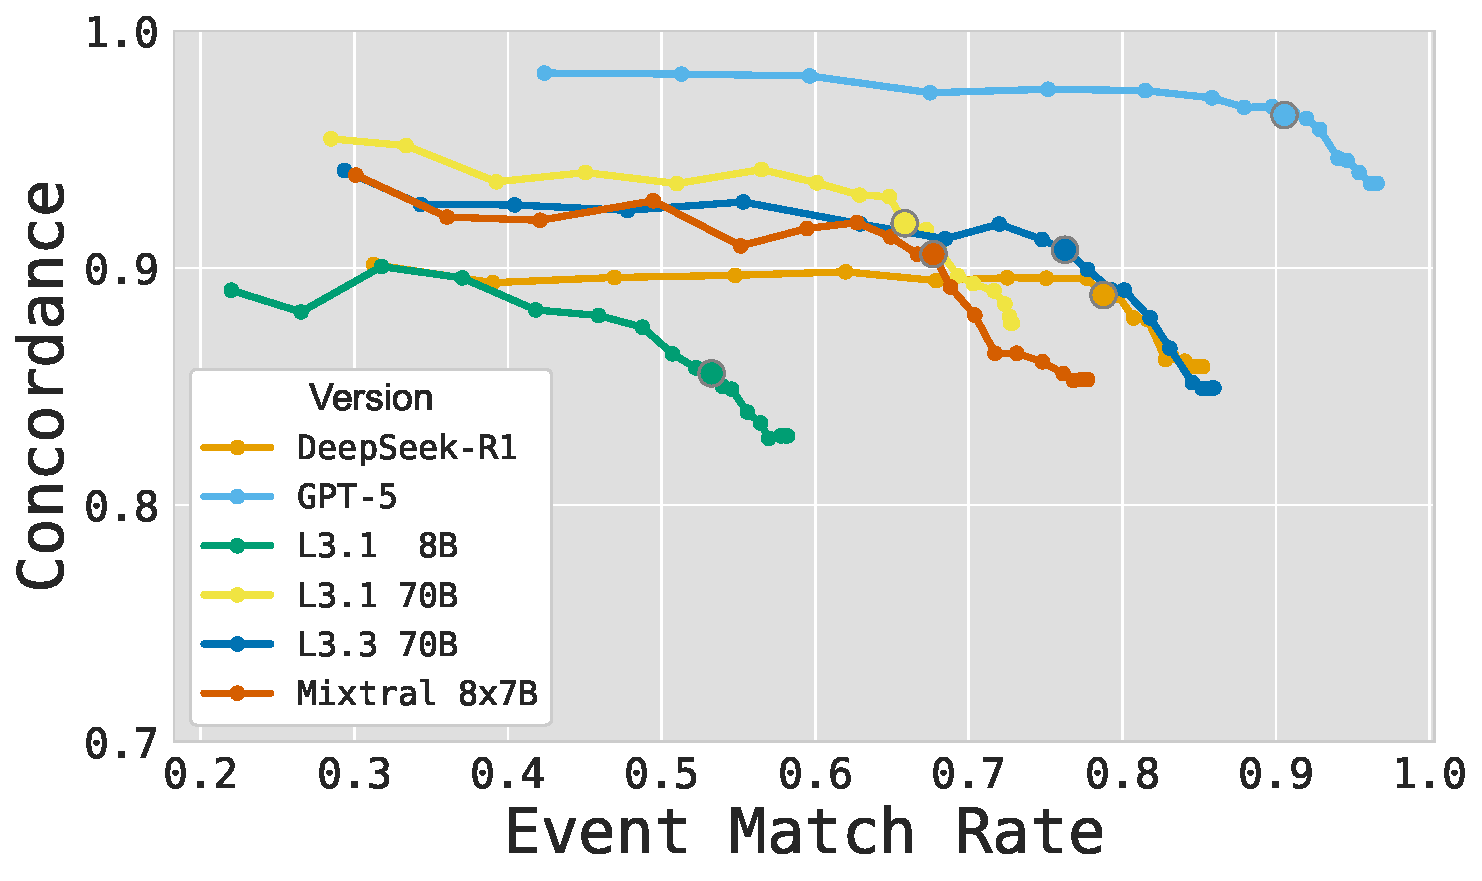
\includegraphics[width=\linewidth]{Appendices/appendix-ch06/images/figures/apd_figs/concordance_vs_event_match_rate.pdf}
        
    \end{minipage}\hfill
    \begin{minipage}[t]{0.48\columnwidth}
        \centering
        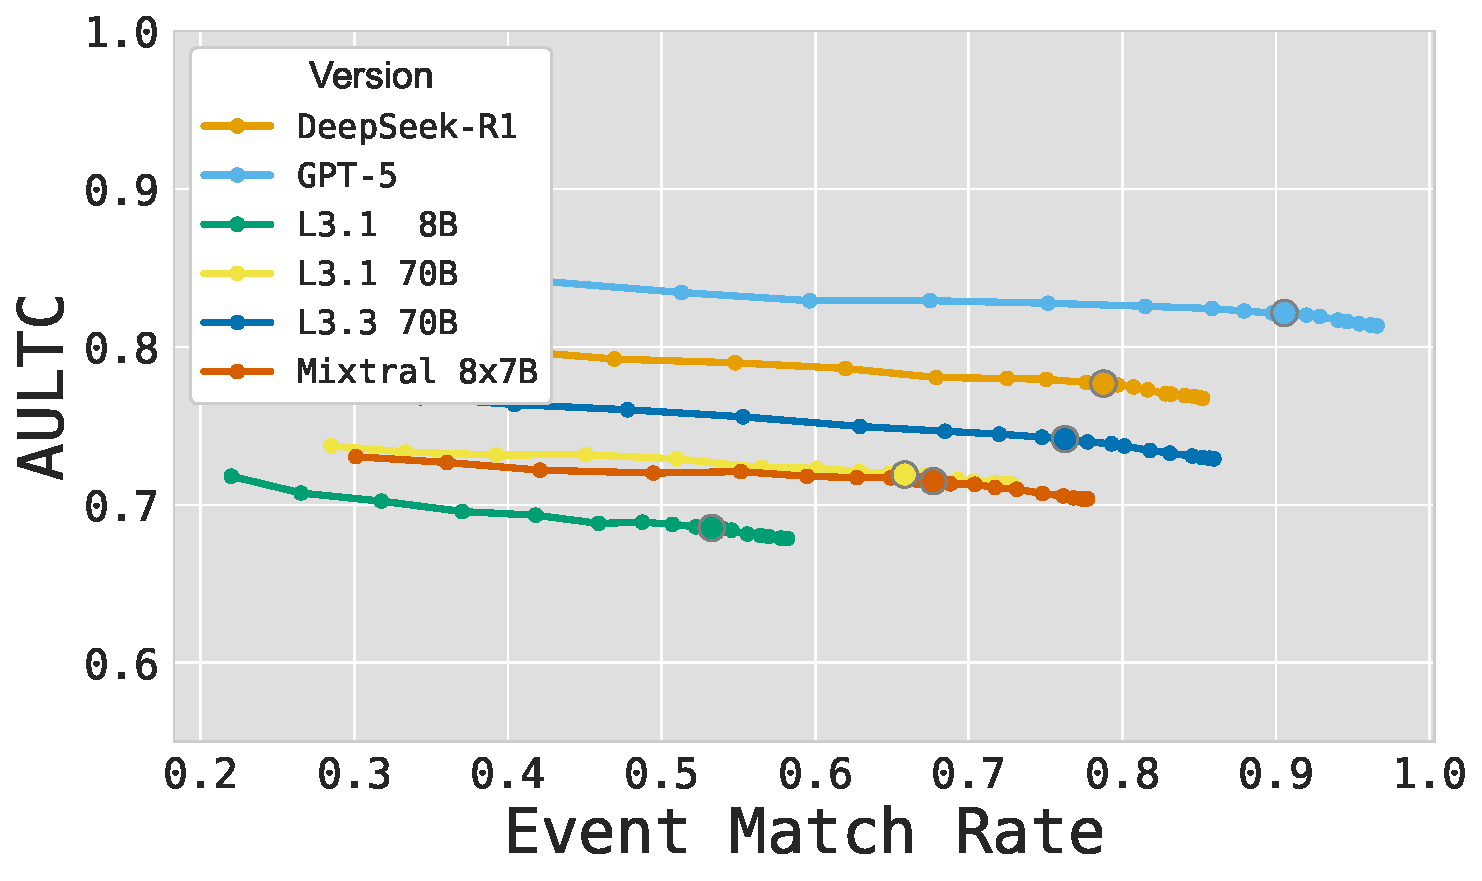
\includegraphics[width=\linewidth]{Appendices/appendix-ch06/images/figures/apd_figs/aultc_vs_event_match_rate.pdf}
    \end{minipage}
    
    

\end{ChSixFloatBody}
\caption{Sensitivity of temporal metrics to the cosine distance threshold $\theta$ for the recursive matching heuristic. Left: Concordance versus event match rate obtained by sweeping $\theta$ in increments of $0.01$ over $[0.01, 0.50]$. Right: AULTC versus event match rate under the same sweep. Each point ($\cdot$) corresponds to a distinct threshold value; the solid large circle ($\bullet$) denotes the threshold $\theta = 0.10$ used throughout the paper.}\ChSixFloatLabel{ch06:fig:threshold_sweep}
\ChSixUncaptionedPanelLabel{ch06:fig:threshold_sweep:concordance}
\ChSixUncaptionedPanelLabel{ch06:fig:threshold_sweep:aultc}
\end{figure}